\documentclass[border=1mm,tikz,preview]{standalone}

\usetikzlibrary{calc}

\newcommand{\convexpath}[2]{
[   
    create hullnodes/.code={
        \global\edef\namelist{#1}
        \foreach [count=\counter] \nodename in \namelist {
            \global\edef\numberofnodes{\counter}
            \node at (\nodename) [draw=none,name=hullnode\counter] {};
        }
        \node at (hullnode\numberofnodes) [name=hullnode0,draw=none] {};
        \pgfmathtruncatemacro\lastnumber{\numberofnodes+1}
        \node at (hullnode1) [name=hullnode\lastnumber,draw=none] {};
    },
    create hullnodes
]
($(hullnode1)!#2!-90:(hullnode0)$)
\foreach [
    evaluate=\currentnode as \previousnode using \currentnode-1,
    evaluate=\currentnode as \nextnode using \currentnode+1
    ] \currentnode in {1,...,\numberofnodes} {
-- ($(hullnode\currentnode)!#2!-90:(hullnode\previousnode)$)
  let \p1 = ($(hullnode\currentnode)!#2!-90:(hullnode\previousnode) - (hullnode\currentnode)$),
    \n1 = {atan2(\y1,\x1)},
    \p2 = ($(hullnode\currentnode)!#2!90:(hullnode\nextnode) - (hullnode\currentnode)$),
    \n2 = {atan2(\y2,\x2)},
    \n{delta} = {-Mod(\n1-\n2,360)}
  in 
    {arc [start angle=\n1, delta angle=\n{delta}, radius=#2]}
}
-- cycle
}

\begin{document}

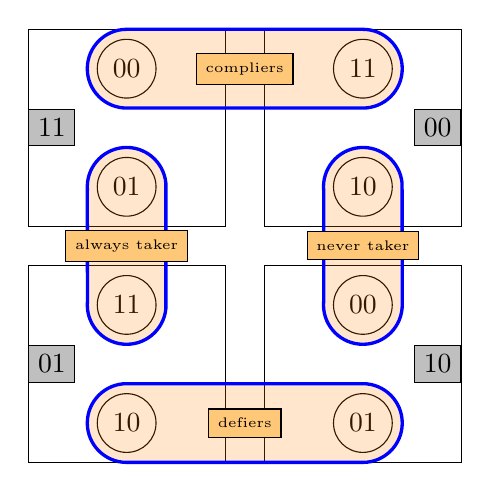
\begin{tikzpicture}[scale=.5]

  \newcommand{\dims}{8}
  \newcommand{\verti}{7}
  \newcommand{\verta}{5}
  \newcommand{\vertb}{2}
  
  \newcommand{\horiz}{6}
  
%% \node (00) at (0, \verti) [circle,draw,radius=1em] {00};

%% \node (01) at (0, \verta) [circle,draw,radius=1em] {01};

%% \node (11) at (0, \vertb) [circle,draw,radius=1em] {11};

%% \node (10) at (0, 0) [circle,radius=1em] {10};

%% \node (11b) at (\horiz, \verti) [circle,draw,radius=1em] {11};

%% \node (10b) at (\horiz, \verta) [circle,draw,radius=1em] {10};

%% \node (00b) at (\horiz, \vertb) [circle,draw,radius=1em] {00};

%% \node (01b) at (\horiz, 0) [circle,draw,radius=1em] {01};

%% \draw[very thick,blue, fill = blue, fill opacity=0.2, draw opacity=1] \convexpath{01,11}{.8cm};

%% \draw[very thick,blue, fill = blue, fill opacity=0.2, draw opacity=1] \convexpath{10,01b}{.8cm};

%% \draw[very thick,blue, fill = blue, fill opacity=0.2, draw opacity=1] \convexpath{00,11b}{.8cm};

%% \draw[very thick,blue, fill = blue, fill opacity=0.2, draw opacity=1] \convexpath{10b,00b}{.8cm};

%% \draw[very thick,orange, fill = blue, fill opacity=0.2, draw opacity=1] \convexpath{00,01}{.8cm};


\draw (1,1) -- (1,6) -- (6, 6) -- (6, 1) -- (1,1);
\draw (7,1) -- (7,6) -- (12, 6) -- (12, 1) -- (7,1);

\draw (1,7) -- (1,12) -- (6, 12) -- (6, 7) -- (1,7);
\draw (7,7) -- (7,12) -- (12, 12) -- (12, 7) -- (7,7);

\node (00) at (3.5, 11) [circle,draw,radius=1em] {00};
\node (01) at (3.5, 8) [circle,draw,radius=1em] {01};

\node (11) at (9.5, 11) [circle,draw,radius=1em] {11};
\node (10) at (9.5, 8) [circle,draw,radius=1em] {10};

\node (11b) at (3.5, 5) [circle,draw,radius=1em] {11};
\node (10b) at (3.5, 2) [circle,draw,radius=1em] {10};

\node (00b) at (9.5, 5) [circle,draw,radius=1em] {00};
\node (01b) at (9.5, 2) [circle,draw,radius=1em] {01};


\draw[very thick,blue, fill = orange, fill opacity=0.2, draw
  opacity=1] \convexpath{00,11}{1cm};
\draw[very thick,blue, fill = orange, fill opacity=0.2, draw
  opacity=1] \convexpath{01,11b}{1cm};
\draw[very thick,blue, fill = orange, fill opacity=0.2, draw
  opacity=1] \convexpath{10b,01b}{1cm};
\draw[very thick,blue, fill = orange, fill opacity=0.2, draw
  opacity=1] \convexpath{00b,10}{1cm};


\node (11c) at (1.6, 9.5) [rectangle,draw,radius=1em, fill=lightgray] {11};
\node (00c) at (11.4, 9.5) [rectangle,draw,radius=1em, fill=lightgray] {00};

\node (01c) at (1.6, 3.5) [rectangle,draw,radius=1em, fill=lightgray] {01};
\node (10c) at (11.4, 3.5) [rectangle,draw,radius=1em, fill=lightgray] {10};

\node (comp) at (6.5, 11) [rectangle,draw,radius=1em, fill =
  {rgb:orange,1;yellow,2;pink,5}] {\tiny compliers};
\node (def) at (6.5, 2) [rectangle,draw,radius=1em, fill =
  {rgb:orange,1;yellow,2;pink,5}] {\tiny defiers};

\node (nt) at (9.5, 6.5) [rectangle,draw,radius=1em, fill =
  {rgb:orange,1;yellow,2;pink,5}] {\tiny never taker};

\node (at) at (3.5, 6.5) [rectangle,draw,radius=1em, fill =
  {rgb:orange,1;yellow,2;pink,5}] {\tiny always taker};


\end{tikzpicture}

\end{document}
